\subsection{Preventivo fase di Progettazione}

\subsubsection{Divisione oraria}
La seguente tabella rappresenta la distribuzione oraria dei ruoli per ogni componente del gruppo:
\rowcolors{2}{\evenRowColor}{\oddRowColor}
\renewcommand{\arraystretch}{2}
\begin{longtable}[h!] { C{3.5cm} C{1cm} C{1cm} C{1cm} C{1cm} C{1cm} C{1cm} C{2cm}}
\caption{Tabella della divisione oraria della Progettazione}\\
\rowcolor{\primaryColor}

\textcolor{\secondaryColor}{\textbf{Membro del gruppo}} & 
\textcolor{\secondaryColor}{\textbf{RE}} & 
\textcolor{\secondaryColor}{\textbf{AM}} & 
\textcolor{\secondaryColor}{\textbf{AN}} & 
\textcolor{\secondaryColor}{\textbf{PT}} & 
\textcolor{\secondaryColor}{\textbf{PR}} & 
\textcolor{\secondaryColor}{\textbf{VE}} & 
\textcolor{\secondaryColor}{\textbf{Ore complessive}}\\	
\endhead
        
\AW{}                     & 10  & - & - & 8 & 8 & 5 & 31 \\
\AT{}                     & -  & 10 & - & 7 & - & 14 & 31 \\
\AD{}                     & -  & 10 & - & 7 & 9 & 9 & 35 \\
\EC{}                     & 11  & - & 6 & - & 9 & 8 & 34 \\
\EM{}                     & -  & - & 7 & 7 & 11 & 9 & 34 \\
\FP{}                     & -  & - & 6 & 10 & 10 & 7 & 33 \\
\GG{}                     & -  & - & 5 & 10 & 11 & 7 & 33 \\
\textbf{Ore totali ruolo} & 21 & 20 & 24 & 49 & 58 & 59 & 231 \\

		
\end{longtable}

\begin{figure}[h!]
    \centering
	\caption{Istogramma relativo alle ore preventivate per ciascun componente nella fase di progettazione}
    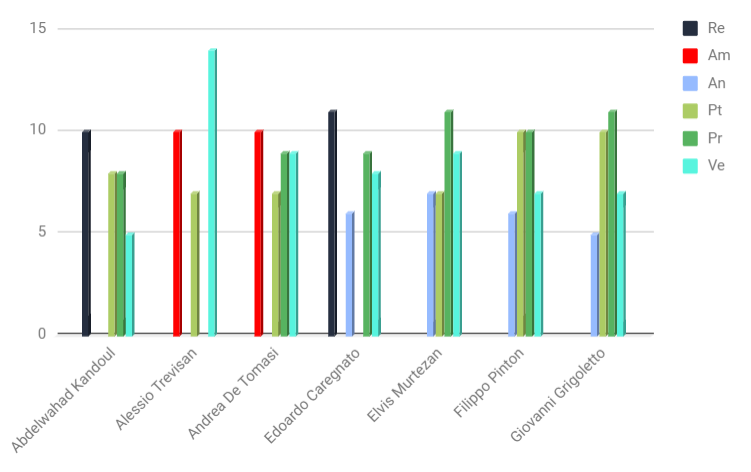
\includegraphics[scale=0.60]{./src/Preventivo/src/img/IstoProj.png}  
\end{figure}
\subsubsection{Preventivo incrementi}
Il preventivo orario parziale degli incrementi non è stato fatto, visto che quello individuato nella \hyperlink{TabellaIncrementi}{tabella degli incrementi} è unico.

\subsubsection{Costo risultante}
La seguente tabella rappresenta per ogni ruolo le ore totali preventivate ed il corrispondente costo in euro:
{
\rowcolors{2}{\evenRowColor}{\oddRowColor}
\renewcommand{\arraystretch}{2}
\begin{longtable}{ C{3cm} C{2cm} C{4cm}}
\caption{Tabella del costo risultante della Progettazione}\\
\rowcolor{\primaryColor}

\textcolor{\secondaryColor}{\textbf{Ruolo}} & 
\textcolor{\secondaryColor}{\textbf{Totale ore}} & 
\textcolor{\secondaryColor}{\textbf{Costo ruolo (in \euro{})}}\\	
\endhead
        
Responsabile    &  21 &  630 \\
Amministratore  &  20 &  400 \\
Analista        &  24 &  600 \\
Progettista     &  49 &  1078 \\
Programmatore   &  58 &  870 \\
Verificatore    &  59 &  885 \\
\textbf{Totale} &  231 & 4463 \\	
        	
\end{longtable}
}

\begin{figure}[h!]
    \centering
	\caption{Areogramma relativo alla quantità di ore totali preventivate per ciascun ruolo nella fase di progettazione}
    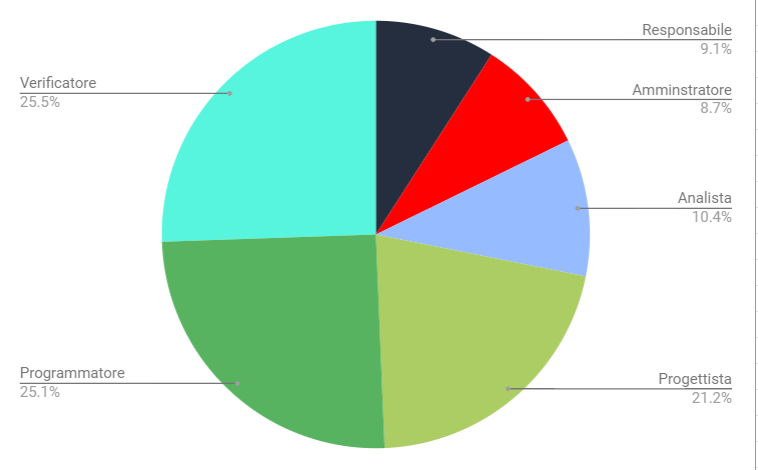
\includegraphics[scale=0.50]{./src/Preventivo/src/img/TortaProj.png}  
\end{figure}
